\documentclass{article}
\usepackage{graphicx} % Required for inserting images
\usepackage{amsmath}
\usepackage{biblatex}
\addbibresource{sources.bib}

\title{Minimizing Crossings}
\author{Noah Albright}
\date{April 2024}

\begin{document}

\maketitle

\section*{Introduction}

Many of the major problems in graph theory today concern minimizing a graph with respect to specific criteria or finding some sort of minimum feature in a graph. One of these features for graph visualization is the crossing number of graph G, which is defined by  

\[ Cr(G) = \sum_{i = 1}^{m-1}{\sum_{j = i+1}^{m}{cross(e_i, e_j)}}\]
\[ \text{With } cross(e, e') = \begin{cases}
    0 & \text{if there is no common point or the common point is an endpoint of both} \\
    1 & \text{if there is one common point that is an interior point of both} \\
    n & \text{if there is overlap between the two edges.}
\end{cases}\]

The main question of my project is: can we predict the rectilinear crossing number of a random graph given the number of edges, nodes, the maximum edge length, minimum edge length, and the closed annulus that contains the graph? We can hopefully use these features to predict the crossing number of a random graph and then use that prediction to try and create an idea to plot a set of edges to a set of points.  

\section*{Relevant Works}
Now, the rectilinear crossing number of a graph has many graph theorists working on conjectures and theorems on the idea. Even the famous mathematician Paul Erdös, in the book \textit{Combinatorics, Geometry and Probability: A Tribute to Paul Erdös} which is a collection of Paul Erdös' favorite problems in mathematics that have been solved or are being worked on at the time. In one chapter, it talks about the rectilinear crossing number and also a connection to a question in probabilistic geometry. \cite{Wilf_1997}  

Now, as mentioned in the proposal, is the paper on the rectilinear crossing number for complete graphs for $K_{5}$ through $K_{27}$. \cite{ABREGO2008261} Another paper gives an upper bound for the  rectilinear crossing number for a complete graph $K_{n}$ given  by

\[ Cr(K_{n} \leq \frac{7n^4 - 56n^3 + 128n^2 -48n[\frac{n-7}{3}] + 108}{432}.\]\cite{JENSEN1971212}

Also, a paper similar to what I am doing proposes a deterministic $n^{2 + o(1)}$ time algorithm to predict the rectilinear crossing number of any n-vertex graph with Cr(G) having $(1 + o(1))\overline{Cr}(G)$ with  $\overline{Cr}(G)$ being the minimum rectilinear number of G.\cite{FOX201945}
As you can see, most of the research on rectilinear crossing numbers has been based heavily on pure math, and so one novelty of my system will be using statistics and data science to predict the rectilinear crossing number. Another thing is that there is a heavy focus on complete graphs, which, even though most of my research will be using complete graphs, when  I make my model I will focus on any graph with any number of edges that is greater than or equal to the number of nodes.  

\section*{Methods}
My project is broken up into 7 different phases, with phase 0 being data collection and the next five phases looking at each of the features closely to see how they correlate with the crossing number of the graph and if we need to square, log, or use some other function on that value to make a linear regression or make sense of the variables.

For phase 0, I first made a C file and shell file to make 1,000 different graphs for each of the other 6 phases. Also, throughout each of the other phases, I will normalize the values based on their maximum values so that when we compare them, we do not compare a $10^6$ crossing number to a $10^{-2}$. Now, why did I do this by the maximum and not the z-score will be given in Appendix D.

For the first phase, I looked at nodes and edges together, as there was no way to look at nodes without changing the number of edges at the same time. So we took the two together and made the graphs to look at how they correlated with the crossing number, and then made a linear regression using the method of least squares with sklearn's linear model library. I will then verify the regression with scoring against the test data for this phase.

Now for the second phase, I looked at the minimum and maximum edge distance in the graph, and similar to phase 1, I will first look at the scatter plot of each feature to see if they correlate with the crossing number and if they need to do a function. Then, once I am finished make and test the linear regression model.

The third and fourth phases are similar to phases 1 and 2, but instead of looking at two features instead, I will look at 1 feature. For phase 3, it was the outer radius and inner radius; for phase 4. Now, for phase 5, I will look at the inner and outer radii combined to see if a combination of the two affects the crossing number with the same steps outlined in phases 1 and 2.

For the final phase, I will take the information from the first 5 phases and make my training and test sets on the random graphs. I will then train three linear regressions using sklearn's LinearRegression, Ridge, and  LASSO regressions. For the  LinearRegression regression, I will find the best subset on the training data and then test it with that same subset of the test data. For the Ridge and LASSO regressions, I will find the $\alpha$ values that will make the best regression on our training data and then test them on our testing data. Once all three are finished testing, we select the best model based on $R^2$ and the mean squared error to be our predictor for the crossing number of a random graph.

\section*{Results}
\renewcommand{\figurename}{Plot}
Now I will get the results for each phase except phase 0, as it was the data collection phase. For phase 1, I first looked at the comparison between edges and nodes, and as shown in Plot 1, they are very correlated but non-linear. So, as the formula for crossings goes for O(edges squared), I squared the edges to get Plot 2, which is a strongly correlated linear scatter plot.

\begin{figure}[!htp]
    \centering
    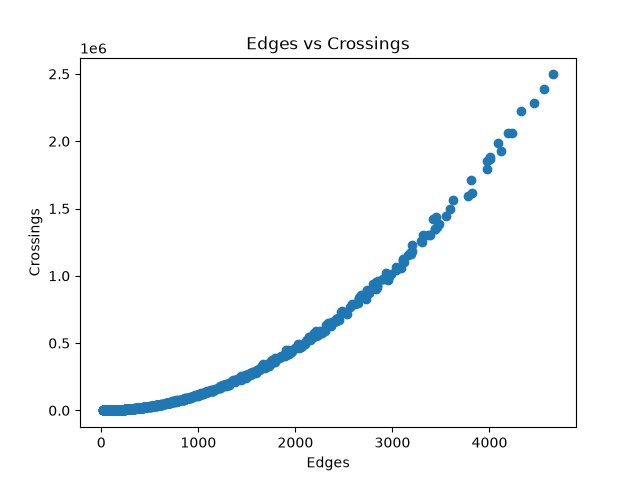
\includegraphics[width = 70mm, height = 40mm]{../figures/graph1.png}
    \caption{edges vs crossings}
    \label{fig:enter-label}
\end{figure}

\begin{figure}[!htp]
    \centering
    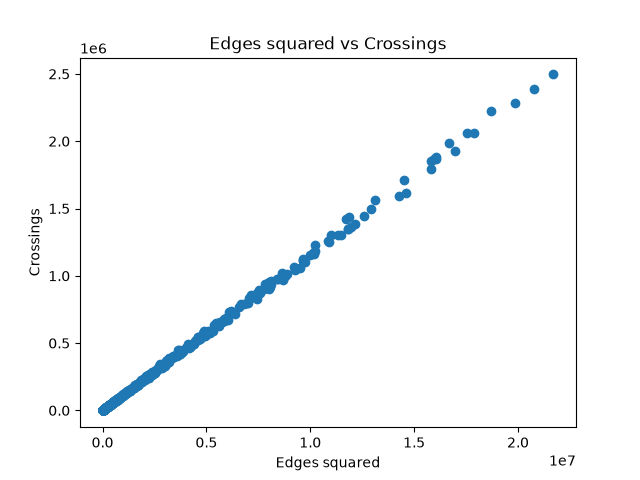
\includegraphics[width = 70mm, height = 40mm]{../figures/graph2.png}
    \caption{edges squared vs crossings}
    \label{fig:enter-label}
\end{figure}

Also, for phase 1 for nodes, I got an upper-bound correlation, which isn't too surprising, as stated in the related works is that there is already a known upper bound for a complete graph, so using that, we will put nodes to the fourth and get Plot 3, with edges being the color gradient for the plot.

\begin{figure}[!htp]
    \centering
    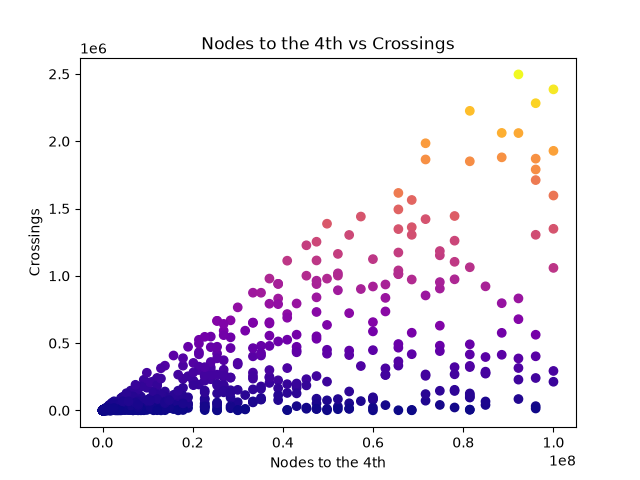
\includegraphics[width = 70mm, height = 40mm]{../figures/graph5.png}
    \caption{nodes to the fourth vs crossings}
    \label{fig:enter-label}
\end{figure}

Now, for phase 1, as you can see from the scatter plots, we got a highly correlated linear regression between the edges and nodes with the crossing number, with an $R^2$ of $.999$ on the training data and $R^2$ of $.992$ on the testing data.

For phases 2 and 3, all my scatter plots given by Plots 4, 5, and 6 have shown no correlation with the data, which is also shown in relatively small $R^2$ scores that are near 0 for the training data and in the negatives for the testing data.

\begin{figure}[!htp]
    \centering
    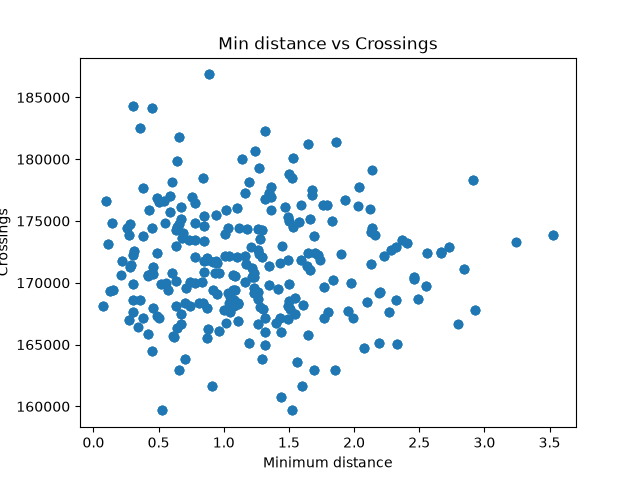
\includegraphics[width = 70mm, height = 40mm]{../figures/graph6.png}
    \caption{min distance vs crossings}
    \label{fig:enter-label}
\end{figure}

\begin{figure}[!htp]
    \centering
    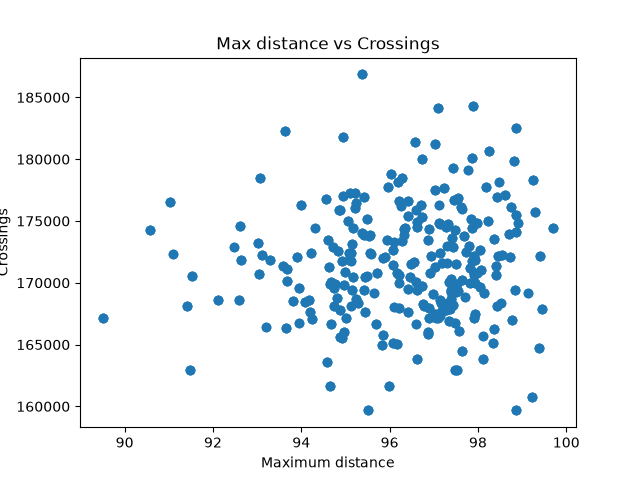
\includegraphics[width = 70mm, height = 40mm]{../figures/graph7.png}
    \caption{max distance vs crossings}
    \label{fig:enter-label}
\end{figure}

\begin{figure}[!htp]
    \centering
    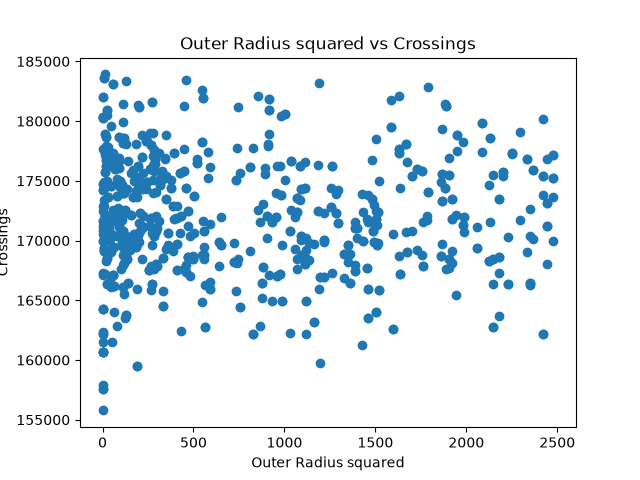
\includegraphics[width = 70mm, height = 40mm]{../figures/graph10.png}
    \caption{outer radius squared vs crossings}
    \label{fig:enter-label}
\end{figure}
\clearpage

Now the fourth phase on the inner radius is different. In this phase, the plot for inner radius vs crossing number given by Plot 7 gives a cool-looking horn shape, implying some sort of correlation. So, as this is the inner radius of the inner circle, I squared the inner radius and got a much more linear plot in Plot 8.

\begin{figure}[!htp]
    \centering
    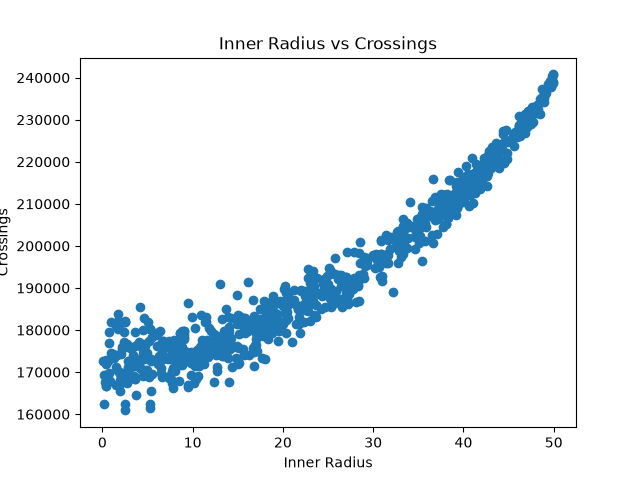
\includegraphics[width = 70mm, height = 40mm]{../figures/graph11.png}
    \caption{inner radius vs crossings}
    \label{fig:enter-label}
\end{figure}

\begin{figure}[!htp]
    \centering
    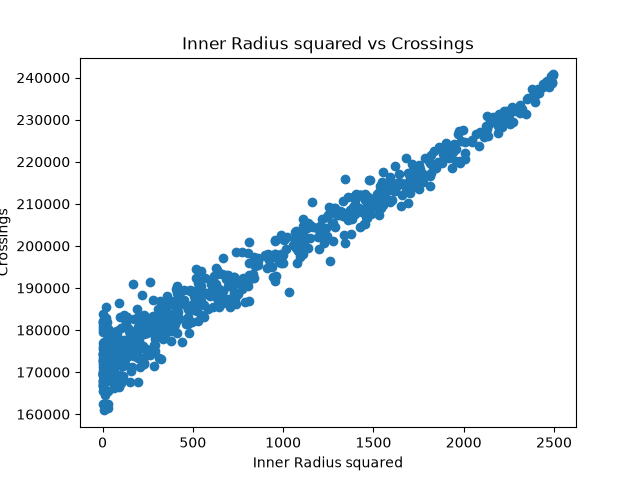
\includegraphics[width = 70mm, height = 40mm]{../figures/graph12.png}
    \caption{inner radius squared vs crossings}
    \label{fig:enter-label}
\end{figure}

Similar to phase 1, I got a linear regression for the inner radius squared to the crossing number of the graph, which got an  $R^2$ of .966 on the training data and an $R^2$ of $.965$ on the testing data. I was surprised at that because we thought it would be a little lower, looking at the variance when it is lower, but we guess it is still very well correlated.

Now for phase 5, we combined phases 3 and 4, which I am noting to show every plot, but Plot 9 shows the inner radius squared vs crossings, with the color map being the outer radius squared. The other plot that we are going to show is the outer radius squared minus the inner radius squared vs crossings in Plot 10, as we are going to add the outer radius minus the inner radius to the features for phase 6.

\begin{figure}[!htp]
    \centering
    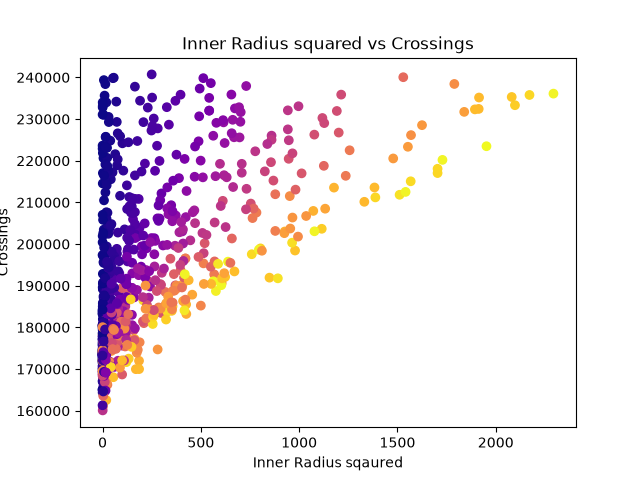
\includegraphics[width = 70mm, height = 40mm]{../figures/graph15.png}
    \caption{inner radius squared vs crossings}
    \label{fig:enter-label}
\end{figure}

\begin{figure}[!htp]
    \centering
    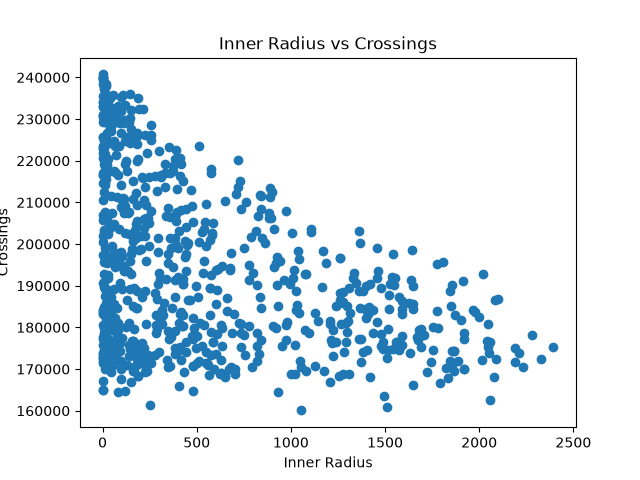
\includegraphics[width = 70mm, height = 40mm]{../figures/graph16.png}
    \caption{outer radius squared - inner radius squared vs crossings}
    \label{fig:enter-label}
\end{figure}

For phase 5, as we can see from the plots, there is not a strong correlation but still some correlation, which is why we got an $R^2$ of .549 on the training data and $R^2$ of .521 on the testing data, meaning they are correlated but not as much as phase 1 and phase 4.

Now for the finishing phase, we trained three different linear regression models from sklearn: LinearRegression, Ridge, and LASSO. For LinearRegression, we looked at every non-empty subset of features to find the subset of features that gave the greatest $R^2$ value, which was the subset of nodes, edges, inner radius, and outer radius with $R^2 = .987$. For Ridge, we tried to find the best $\alpha$ value that gave the maximum $R^2$, which was $\alpha = 0.1$ with $R^2 = .986$. Now for LASSO, we tried to find the best $\alpha$ value that gave the minimum mean squared error, which was $\alpha = 7.11 \times 10^{-5}$ with a mean squared error of $0.0004$.

For the final part, I tested each of the three trained linear models on the testing data for phase  6. For LinearRegression, I got an $R^2$ of $.988$ and a mean squared error of $.0003$; For Ridge, I got an $R^2$ of $.987$ and a mean squared error of $.0003$; And for LASSO, I got an $R^2$ of $.988$ and a mean squared error of $0.0003$.So, all three regressions did well at predicting the rectilinear crossing number that I will state all three.Let n = nodes, e = edges, r = inner radius, R = outer radius, m = minimum distance, and M = maximum distance; then

\[\text{LinearRegression: } Cr(G) = 0.006n^4 + 1.029e^2 + 0.046r^2 -0.013R^2\],
\[\text{Ridge: } Cr(G) = 0.018n^4 + 0.995e^2 +0.02r^2 -0.003R^2 +0.005m + 0.017M -0.023(R^2 - r^2)\], and
\[\text{LASSO: } Cr(G) = 0.007n^4 + 1.026e^2 +0.029r^2 +0.002M -0.013(R^2 - r^2)\].


\section*{Conclusion}
Going through this project was a lot of work, especially for many features that were not very correlated with the rectilinear crossing number of a graph. The one thing I will conclude from this project is that for any graph, it is probably best to look at the number of edges and square it to predict the rectilinear crossing number of a graph. It also explains why there is not much data science on this topic either, as there is nothing much that data can give you besides looking at how many edges you have.

Now one thing I do want to look at further from my data is the inner radius feature and how they compare with the rectilinear crossing number. The inner radius, it was correlated, but I stated in the paper and the notebook that as it increases, the less variance it has, so maybe we can research further why it is. Also, just as I finish up this paper, another idea is to divide it by the outer radius to see if that is in any way correlated to the rectilinear crossing number.

Overall, this project was a lot of fun but stressful, as basically, the answer was clear based on the research done on this subject, but I had some ideas I wanted to try and find an answer to those ideas. So, in the fall semester, I am taking a Graph theory course, and we have a topic on the crossing numbers of a graph, and maybe apply more knowledge later.  

\section*{Appendices}

\subsection*{Appendix A - makeData. c and makeData.sh}

You will notice that I have included a makeData.c and makeData.sh files with my notebook, which, as the name of the files suggests, are the files that made all my data for this project. Now you don't have to run them, but if you want to know how I got my data, then they are included with my notebook submission (also, I don't want to include 500 lines of C code in my notebook). Also, some of the appendices are about some stuff that happens in makeData.c.

\subsection*{Appendix B - makeData.c random edges}
So in the makeData.c, you will see the comment in my makeEdges function to explain why the deterministic way that I made the edges is still random, as it is not obvious why it will be (or at least to me anyway). The edges are random because the nodes (points) that make up the edges are random, and thus even in the deterministic way that I made them, it will be random. 

For example, take me throwing n different dice, with each having a random number of sides; then we remove the last half of the dice that we threw. Now we selected n/2 dice, which is random, as we didn't know which die would be going at the kth position for $1 \leq k \leq n$. So, as this example shows, we can have the process to remove be deterministic while it still creates a random selection. 

\subsection*{Appendix C - makeData.c getCross}
Also, in the makeData.c  you will see in the function comment on the crossings, cross, and getCross function that more on those functions will be given in the paper. Now, the first should be self-explanatory by the introduction to the paper, so I will not be going over those two; instead, we will focus on getCross and how it finds which of the three options our two edges are.

The main idea is that a rectilinear cross is just solving a system of linear equations between the two edges. For the first part of my code, it just checks if the edges are first parallel and if they lie on the same line. Between those two and some distance checking, we can see if they have some sort of overlap: option 2 or none at all 0. After passing through the first part, we can guarantee a single unique solution to the system. Now there are many ways to solve the linear equation, like row reduction or Cramer's rule (tried this originally) but row reduction is hard to do for a computer, and Cramer's rule was not working with my code. So I just solved the system just as I would have in high school which let $a_{1}x + b_{1}x = c_{1}$ and $a_{2}x + b_{2}x = c_{2}$ be the two linear equations with assume that $a_{1} \neq 0$. Then the unique solution to the system is 
\[  y = \frac{c_{2} - c_{1} * \frac{a_{2}}{a_{1}}}{b_{2} - b_{1}} * \frac{a_{2}}{a_{1}}\]
\[  x =  \frac{c_{1} - b_{1}y}{a_{1}}.\]

Now, for $a_{1} = 0$, we just flip the order we solve for x and y, which will result in the code given in getCross. 


\printbibliography

\end{document}
